\newpage
\section{Auswertung} % (fold)
\label{sec:auswertung}

Für die nachfolgende Auswertung werden die Eigenschaften von Kupfer aus Tabelle \ref{Eigenschaften} verwendet.

\begin{table}[!h]
	\centering
	\caption[]{Eigenschaften von Kupfer \cite{kupfer1}\cite{kupfer2}.}
	\begin{tabular}{rrrrr}
		\toprule
		Masse/$\si{\gram}$ & Molmasse/$\si{\gram\per\mol}$ & $\rho \cdot 10^6/\si{\gram\per\meter^3}$ & $\Kappa \cdot 10^9/\si{\pascal}$ & $V_0 \cdot 10^{-6}/\si{\meter^3\per\mol}$\\
		\midrule
		342 & 63,546 & 8,92 & 7,11 & 140\\
		\bottomrule
	\end{tabular}
	\label{Eigenschaften}
\end{table}

\FloatBarrier
\subsection{Bestimmung der Molwärme $C_V$} % (fold)
\label{sub:bestimmung_von_c__mathrm}

\begin{table}[!h]
	\caption[]{Ergebnisse bei der Bestimmung von $C_V$.}
	\centering
	\begin{tabular}{S[table-format=3.2(2)] S[table-format=2.1(1)] S[table-format=2.1(1)] S[table-format=2.1(1)]}
\toprule
\multicolumn{1}{c}{$T/\si{\kelvin}$} & \multicolumn{1}{c}{$C_p/\si{\joule\per\mol\per\kelvin}$} & \multicolumn{1}{c}{$\alpha \cdot 10^{-6}/\si{1\per\kelvin}$} & \multicolumn{1}{c}{$C_V/\si{\joule\per\mol\per\kelvin}$}\\
\midrule
85.55 \pm 0.17 & 12.4 \pm 0.4 & 9.2 \pm 0.8 & 12.3 \pm 0.4 \\
94.65 \pm 0.17 & 15.8 \pm 0.7 & 10.2 \pm 0.8 & 15.7 \pm 0.7 \\
103.07 \pm 0.17 & 17.5 \pm 0.8 & 11.0 \pm 0.8 & 17.4 \pm 0.8 \\
111.53 \pm 0.17 & 19.0 \pm 0.9 & 11.6 \pm 0.8 & 18.9 \pm 0.9 \\
119.67 \pm 0.17 & 20.0 \pm 0.9 & 12.1 \pm 0.8 & 19.8 \pm 0.9 \\
127.48 \pm 0.17 & 20.9 \pm 1.0 & 12.6 \pm 0.8 & 20.7 \pm 1.0 \\
135.19 \pm 0.17 & 20.7 \pm 1.0 & 12.9 \pm 0.8 & 20.5 \pm 1.0 \\
143.78 \pm 0.17 & 20.6 \pm 0.9 & 13.3 \pm 0.8 & 20.4 \pm 0.9 \\
152.28 \pm 0.17 & 20.6 \pm 0.9 & 13.6 \pm 0.8 & 20.3 \pm 0.9 \\
161.31 \pm 0.17 & 19.4 \pm 0.8 & 13.9 \pm 0.8 & 19.1 \pm 0.8 \\
170.50 \pm 0.17 & 19.9 \pm 0.8 & 14.2 \pm 0.8 & 19.6 \pm 0.8 \\
179.47 \pm 0.18 & 19.9 \pm 0.8 & 14.5 \pm 0.8 & 19.6 \pm 0.8 \\
189.11 \pm 0.18 & 21.0 \pm 0.8 & 14.7 \pm 0.8 & 20.6 \pm 0.8 \\
198.53 \pm 0.18 & 22.2 \pm 1.0 & 14.9 \pm 0.8 & 21.8 \pm 1.0 \\
208.87 \pm 0.18 & 22.0 \pm 4.0 & 15.2 \pm 0.8 & 21.0 \pm 4.0 \\
219.01 \pm 0.18 & 23.0 \pm 5.0 & 15.4 \pm 0.8 & 23.0 \pm 5.0 \\
228.30 \pm 0.18 & 25.0 \pm 5.0 & 15.6 \pm 0.8 & 24.0 \pm 5.0 \\
237.26 \pm 0.18 & 25.0 \pm 6.0 & 15.7 \pm 0.8 & 25.0 \pm 6.0 \\
249.69 \pm 0.18 & 15.9 \pm 3.5 & 15.9 \pm 0.8 & 15.3 \pm 3.5 \\
266.52 \pm 0.18 & 11.8 \pm 2.5 & 16.2 \pm 0.8 & 11.1 \pm 2.5 \\
288.76 \pm 0.18 &  9.0 \pm 0.2 & 16.5 \pm 0.8 &  8.3 \pm 0.2 \\
\bottomrule
\end{tabular}
	\label{Cv}
\end{table}

\begin{table}[!h]
	\centering
	\caption[]{Werte zur Bestimmung von $C_p$.}
	\begin{tabular}{S[table-format=3.2(2)] S[table-format=3.2(2)] S[table-format=3.1(1)] S[table-format=2.3(3)] S[table-format=3.2(2)]}
\toprule
\multicolumn{1}{c}{$R_0/\si{\ohm}$} & \multicolumn{1}{c}{$R_1/\si{\ohm}$} & \multicolumn{1}{c}{$t/\si{\second}$} & \multicolumn{1}{c}{$U/\si{\volt}$} & \multicolumn{1}{c}{$I/\si{\milli\ampere}$}\\
\midrule
21.80 \pm 0.10 & 25.80 \pm 0.10 & 240.0 \pm 0.5 & 16.620 \pm 0.005 & 157.20 \pm 0.05 \\
26.00 \pm 0.10 & 29.30 \pm 0.10 & 300.0 \pm 0.5 & 15.230 \pm 0.005 & 145.40 \pm 0.05 \\
29.60 \pm 0.10 & 32.80 \pm 0.10 & 300.0 \pm 0.5 & 15.840 \pm 0.005 & 151.00 \pm 0.05 \\
33.20 \pm 0.10 & 36.30 \pm 0.10 & 300.0 \pm 0.5 & 16.290 \pm 0.005 & 155.00 \pm 0.05 \\
36.60 \pm 0.10 & 39.70 \pm 0.10 & 300.0 \pm 0.5 & 16.740 \pm 0.005 & 159.10 \pm 0.05 \\
39.90 \pm 0.10 & 42.90 \pm 0.10 & 304.0 \pm 0.5 & 16.780 \pm 0.005 & 159.30 \pm 0.05 \\
43.10 \pm 0.10 & 46.10 \pm 0.10 & 300.0 \pm 0.5 & 16.820 \pm 0.005 & 159.60 \pm 0.05 \\
46.60 \pm 0.10 & 49.70 \pm 0.10 & 300.0 \pm 0.5 & 17.130 \pm 0.005 & 162.40 \pm 0.05 \\
50.00 \pm 0.10 & 53.30 \pm 0.10 & 300.0 \pm 0.5 & 17.690 \pm 0.005 & 167.60 \pm 0.05 \\
53.60 \pm 0.10 & 57.10 \pm 0.10 & 300.0 \pm 0.5 & 17.720 \pm 0.005 & 167.80 \pm 0.05 \\
57.40 \pm 0.10 & 60.80 \pm 0.10 & 300.0 \pm 0.5 & 17.740 \pm 0.005 & 167.90 \pm 0.05 \\
61.00 \pm 0.10 & 64.50 \pm 0.10 & 300.0 \pm 0.5 & 18.040 \pm 0.005 & 170.80 \pm 0.05 \\
64.90 \pm 0.10 & 68.40 \pm 0.10 & 300.0 \pm 0.5 & 18.550 \pm 0.005 & 175.60 \pm 0.05 \\
68.80 \pm 0.10 & 72.10 \pm 0.10 & 300.0 \pm 0.5 & 18.560 \pm 0.005 & 175.80 \pm 0.05 \\
72.70 \pm 0.10 & 76.50 \pm 0.10 & 300.0 \pm 0.5 & 18.560 \pm 3.000 & 197.60 \pm 0.05 \\
76.90 \pm 0.10 & 80.40 \pm 0.10 & 300.0 \pm 0.5 & 18.560 \pm 4.000 & 197.70 \pm 0.05 \\
80.70 \pm 0.10 & 84.00 \pm 0.10 & 300.0 \pm 0.5 & 18.560 \pm 4.000 & 197.80 \pm 0.05 \\
84.10 \pm 0.10 & 87.70 \pm 0.10 & 337.0 \pm 0.5 & 18.560 \pm 4.000 & 197.70 \pm 0.05 \\
88.10 \pm 0.10 & 93.50 \pm 0.10 & 320.0 \pm 0.5 & 18.560 \pm 4.000 & 197.90 \pm 0.05 \\
94.00 \pm 0.10 & 100.80 \pm 0.10 & 300.0 \pm 0.5 & 18.560 \pm 4.000 & 197.90 \pm 0.05 \\
102.80 \pm 0.10 & 109.30 \pm 0.10 & 300.0 \pm 0.5 & 16.860 \pm 0.005 & 160.10 \pm 0.05 \\
\bottomrule
\end{tabular}
	\label{Daten}
\end{table}

Die Ergebnisse zur Bestimmung von $C_V$ sind in Tabelle \ref{Cv} dargestellt.
$C_p$ konnte über
\begin{equation*}
	C_p = \frac{M Q}{m \Delta T} = \frac{M t U I}{m \Delta T}
\end{equation*}
berechnet werden \ref{Daten}.
Dabei ist der Fehler durch
\begin{equation*}
	\Delta C_p = \sqrt{\left(|\frac{\partial C_p}{\partial t}|\cdot \Delta t \right)^2 + \left(|\frac{\partial C_p}{\partial U}|\cdot \Delta U \right)^2 + \left(|\frac{\partial C_p}{\partial I}|\cdot \Delta I \right)^2 + \left(|\frac{\partial C_p}{\partial \Delta T}|\cdot \Delta (\Delta T) \right)^2}
\end{equation*}

Die Temperatur in Kelvin ist aus dem Widerstand mithilfe der Gleichung
\begin{equation*}
	T(R) = \SI{0.00137}{\kelvin\per\ohm^2} \cdot R^2 + \SI{2.296}{\kelvin\per\ohm} \cdot R + \SI{30.194 \pm 0.017}{\kelvin}
\end{equation*}
berechnet worden, welche aus einer nicht-linearen Regression mithilfe der Methode der kleinsten Quadrate der Werte aus Tabelle \ref{Temperatur} gewonnen worden ist.
Die Vorfaktore von $R^2$ und $R$ haben dabei vernachlässigbar kleine Fehler.

\begin{table}[!h]
	\centering
	\caption[]{Temperatur in Abhängigkeit des Widerstandes \cite{V47}.}
	\begin{tabular}{S[table-format=3.2] S[table-format=2.2] S[table-format=3.2] S[table-format=3.2]}
\toprule
\multicolumn{1}{c}{$T/\si{\kelvin}$} & \multicolumn{1}{c}{$R/\si{\ohm}$} & \multicolumn{1}{c}{$T/\si{\kelvin}$} & \multicolumn{1}{c}{$R/\si{\ohm}$}\\
\midrule
 73.15 & 18.44 & 193.15 &  68.28 \\
 83.15 & 22.71 & 203.15 &  72.29 \\
 93.15 & 27.03 & 213.15 &  76.28 \\
103.15 & 31.28 & 223.15 &  80.25 \\
113.15 & 35.48 & 233.15 &  84.21 \\
123.15 & 39.65 & 243.15 &  88.17 \\
133.15 & 43.80 & 253.15 &  92.13 \\
143.15 & 47.93 & 263.15 &  96.07 \\
153.15 & 52.04 & 273.15 & 100.00 \\
163.15 & 56.13 & 283.15 & 103.90 \\
173.15 & 60.20 & 293.15 & 107.79 \\
183.15 & 64.25 & 303.15 & 111.67 \\
\bottomrule
\end{tabular}
	\label{Temperatur}
\end{table}

$C_V$ lässt sich nun aus Gleichung \eqref{eqn:cp_cv} 
berechnen.
Dabei ist der Fehler durch
\begin{equation*}
	\Delta C_V = \sqrt{\left(|\frac{\partial C_V}{\partial C_p}|\cdot \Delta C_p \right)^2 + \left(|\frac{\partial C_V}{\partial \alpha}|\cdot \Delta \alpha \right)^2 + \left(|\frac{\partial C_V}{\partial T}|\cdot \Delta T \right)^2}
\end{equation*}
Dazu ist für die Temperatur der Mittelwert aus Anfangs- und Endwiderstand verwendet worden.
Der lineare Ausdehnungskoeffizient ist aus der Temperatur mithilfe der Gleichung
\begin{eqnarray*}
	\alpha(T) = 
	\SI{4.413 e-17}{1\per\kelvin^6} \cdot T^5 +
	\SI{-4.898 e-14}{1\per\kelvin^5} \cdot T^4 + 
	\SI{2.180 e-11}{1\per\kelvin^4} \cdot T^3 +\\ 
	\SI{-4.936 e-9}{1\per\kelvin^3}\cdot T^2 + 
	\SI{5.958 e-7}{1\per\kelvin^2} \cdot T^1 + 
	\SI{-1.687 e-5}{1\per\kelvin} 
\end{eqnarray*}
berechnet worden, welche aus einer nicht-linearen Regression mithilfe der Methode der kleinsten Quadrate der Werte aus Tabelle \ref{Alpha} gewonnen worden ist.
Die Fehler sind vernachlässigbar.

\begin{table}[!h]
	\centering
	\caption[]{$\alpha$ in Abhängigkeit der Temperatur \cite{V47}.}
	\begin{tabular}{S[table-format=3.1] S[table-format=2.2] S[table-format=3.1] S[table-format=2.2]}
\toprule
\multicolumn{1}{c}{$T/\si{\kelvin}$} & \multicolumn{1}{c}{$\alpha \cdot 10^{-6}/\si{1\per\kelvin}$} & \multicolumn{1}{c}{$T/\si{\kelvin}$} & \multicolumn{1}{c}{$\alpha \cdot 10^{-6}/\si{1\per\kelvin}$}\\
\midrule
 70.0 &  7.00 & 190.0 & 14.75 \\
 80.0 &  8.50 & 200.0 & 14.95 \\
 90.0 &  9.75 & 210.0 & 15.20 \\
100.0 & 10.70 & 220.0 & 15.40 \\
110.0 & 11.50 & 230.0 & 15.60 \\
120.0 & 12.10 & 240.0 & 15.75 \\
130.0 & 12.65 & 250.0 & 15.90 \\
140.0 & 13.15 & 260.0 & 16.10 \\
150.0 & 13.60 & 270.0 & 16.25 \\
160.0 & 13.90 & 280.0 & 16.35 \\
170.0 & 14.25 & 290.0 & 16.50 \\
180.0 & 14.50 &  &  \\
\bottomrule
\end{tabular}
	\label{Alpha}
\end{table}

Die Ergebnisse sind graphisch in Abbildung \ref{Cv_gra} dargestellt.
Zudem ist die Theoriekurve nach Gleichung \eqref{eqn:cv_debye} mit dem Theoriewert von $\Theta_D = \SI{345}{\kelvin}$ \cite{kupfer3} errechnet und der Abbildung hinzugefügt worden.

\begin{figure}
	\centering
	\includegraphics[width = 14cm]{build/Cv_Cv.pdf}
	\caption[]{Graphische Darstellung der Ergebnisse von $C_V$ und der dazugehörigen Theoriekurve.}
	\label{Cv_gra}
\end{figure}

\begin{figure}
	\begin{minipage}{8cm}
		\includegraphics[width = 8cm]{build/Cv_Temperatur.pdf}
	\end{minipage}
	\hfill
	\begin{minipage}{8cm}
		\includegraphics[width = 8cm]{build/Cv_alpha.pdf}
	\end{minipage}
	\caption[]{Werte zur Bestimmung der Funktion zur Berechnung der Temperatur $T$ und dem linearen Ausdehnungskoeffizienten $\alpha$ und den dazugehörigen Fit-Funktionen.}
\end{figure}

\subsection{Bestimmung der Debye-Temperatur $\Theta_\mathrm{D}$} % (fold)
\label{sub:bestimmung_der_debye_temperatur_theta_mathrm}

\begin{table}[!h]
	\centering
	\caption[]{Ergebnisse der Berechnung der Debye-Temperatur.}
	\input{build/Theta.tex}
	\label{Theta_Debye}
\end{table}

\begin{figure}[!h]
	\centering
	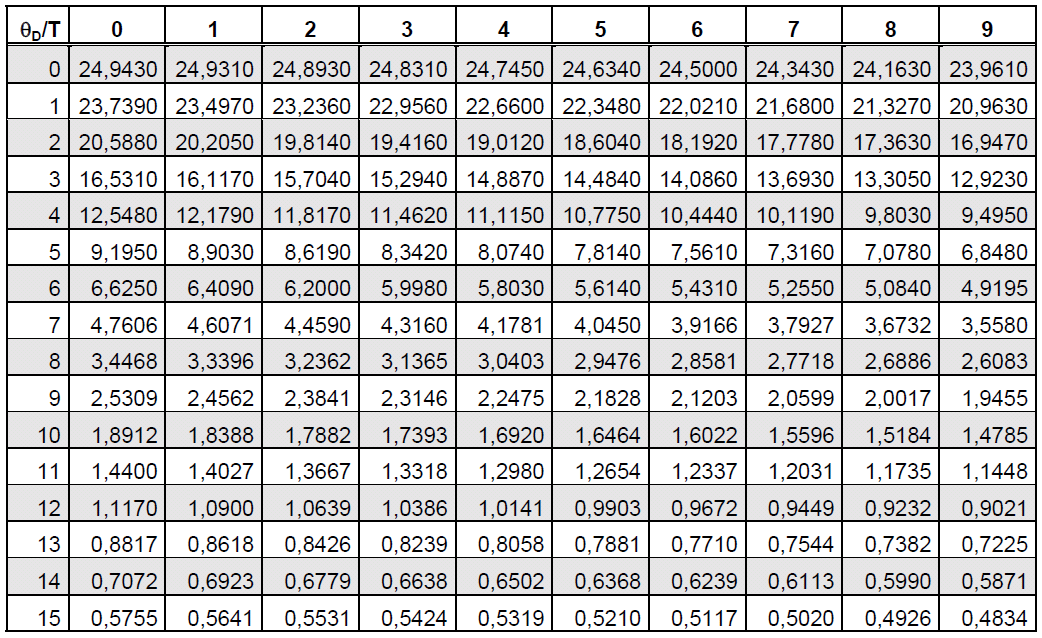
\includegraphics[width = 14cm]{img/theta.png}
	\caption[]{Werte der Universellen Debye-Funktion für $C_V$ zur Bestimmung der Debye-Temperatur $\Theta_\mathrm{D}$ \cite{V47}.}
	\label{Cv_global}
\end{figure}

Beim Vergleich der errechneten Werte von $C_V$ bis zur Temperatur $T_\text{max} = \SI{170}{\kelvin}$ mit der Debye-Funktion aus Tabelle \ref{Cv_global} haben sich die in Tabelle \ref{Theta_Debye} dargestellten Werte für $\Theta_\text{D} / T$ ergeben.
Zudem ist es möglich durch Multiplikation mit der Temperatur auf den Wert für $\Theta_\text{D}$ zu schließen.

Durch Bilden des Mittelwertes der Debye-Temperaturen konnte der Wert $\Theta_\mathrm{D} = \SI{308 \pm 2}{\kelvin}$ errechnet werden.
\FloatBarrier
\subsection{Theoretische Berechnung von $\omega_\mathrm{D}$ und $\Theta_\mathrm{D}$} % (fold)
\label{sub:theoretische_berechnung_von_omega_mathrm}

Mithilfe der Gleichung \eqref{eqn:omega_debye}, den Geschwindigkeiten $v_\text{l}=\SI{4.7}{\kilo\meter\per\second}$ und $v_\text{tr}=\SI{2.26}{\kilo\meter\per\second}$ und dem Zusammenhang
\begin{equation*}
	N = N_\text{A} \frac{m}{M}
\end{equation*}
ergiebt sich \input{omega_D_theo.tex}.
Daraus errechnet sich mithilfe der Gleichung
\begin{equation*}
	\Theta_\text{D} = \frac{\hbar \omega_\text{D}}{\kb}
\end{equation*}
die Debye-Temperatur zu \input{theta_D_theo.tex}.